%
% teil2.tex -- Beispiel-File für teil2 
%
% (c) 2020 Prof Dr Andreas Müller, Hochschule Rapperswil
%
\section{Drehung
\label{clifford:section:drehung}}
\rhead{Drehung}

Eine Drehung kann man aus zwei aufeinanderfolgenden Spiegelungen bilden.
Das kann vielleicht zuerst eine verwirrende Aussage sein, da man aus den vorher gezeigten Formeln annehmen könnte, dass die Spiegelung schon für eine Drehung ausreicht.
Obwohl sich die Längen, Winkel und Volumen sich bei einer Spiegelung wie bei einer Drehung nicht ändert, sind sie doch verschieden, da die Orientierung bei der Spiegelung invertiert wird.
Stellt man sich, wie im Bild \ref{BildSpiegRot} dargestellt, beispielsweise ein Objekt vor und spiegelt dieses an einer Ebene, dann ist es unmöglich, nur durch eine Drehung (egal an welchem Punkt) das ursprüngliche Objekt deckungsgleich auf das Gespiegelte zu drehen.
Hingegen ist es wiederum möglich ein zweifach gespiegeltes Objekt durch eine Drehung zu erreichen.
Das liegt daran, dass die Orientierung zweimal invertiert wurde.
\index{Drehung}%
\index{Orientierung}%

\begin{figure}
	\centering
	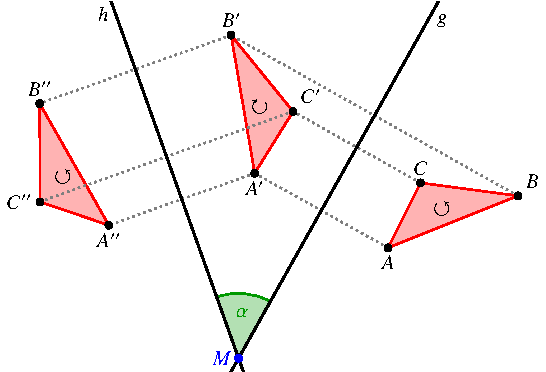
\includegraphics[width=10cm]{papers/clifford/images/spiegelung.pdf}
	\caption{Der wesentliche Unterschied zwischen Spiegelung und Drehung ist die Umkehrung der Orientierung.}
	\label{BildSpiegRot}
\end{figure}

\begin{figure}
	\centering
	\begin{tikzpicture}[>=latex]
	\draw[thin,gray!40] (-3,-1) grid (3,3);
	\draw[->] (-3.1,0)--(3.2,0) node[right]{$a_1$};
	\draw[->] (0,-1.1)--(0,3.2) node[above]{$a_2$};
	\draw[line width=1.0pt,darkgreen,-stealth](2,2)--(-2,2) node[anchor=south west]{$\boldsymbol{-2v_{\parallel u}}$};
	\draw[line width=1.0pt,darkgreen,-stealth](-2,2)--(-2.828,0) node[anchor=north west]{$\boldsymbol{-2v'_{\parallel w}}$};
	\draw[blue, line width=1.0pt] (0,3)--(0,-1) node[anchor=south east]{$\sigma_u$};
	\draw[red, line width=1.0pt] (-3,1.24)--(2.21,-1) node[anchor=south]{$\sigma_w$};
	\draw[line width=2pt,black,-stealth](0,0)--(2,2) node[anchor=south east]{$\boldsymbol{v}$};
	\draw[line width=1.5pt,blue,-stealth](0,0)--(2.5, 0) node[anchor=south east]{$\boldsymbol{u}$};
	\draw[line width=2pt,black,-stealth](0,0)--(-2,2) node[anchor=south east]{$\boldsymbol{v'}$};
	\draw[line width=1.5pt,red,-stealth](0,0)--(0.957, 2.31) node[anchor=south east]{$\boldsymbol{w}$};
	\draw[line width=2pt,black,-stealth](0,0)--(-2.828,0) node[anchor=south east]{$\boldsymbol{v''}$};
	\draw[line width=1.5pt,gray,-stealth](0,0)--(1,0) node[anchor=north]{$\boldsymbol{e_1}$};
	\draw[line width=1.5pt,gray,-stealth](0,0)--(0,1) node[anchor=north east]{$\boldsymbol{e_2}$};
	
	\coordinate (A) at (0,0);
	\coordinate (B) at (2.5,0);
	\coordinate (C) at (0.957, 2.31);
	\tikzset{anglestyle/.style={angle eccentricity=1.25, purple, draw,  thick, angle radius=1cm}}
	\draw pic ["$\vartheta$", anglestyle] {angle = B--A--C};
	\coordinate (D) at (0,0);
	\coordinate (E) at (1,1);
	\coordinate (F) at (-1, 0);
	\tikzset{anglestyle/.style={angle eccentricity=1.25, purple,  draw,  thick, angle radius=1.25cm}}
	\draw pic ["$2\vartheta$", anglestyle] {angle = E--D--F};
	\end{tikzpicture}
	\caption{Drehung des Vektors $\textbf{v}$ um $2\vartheta$}
	\label{BildDrehung}
\end{figure}

\subsection{Drehung in der linearen Algebra}
In der linearen Algebra haben wir Drehungen durch die Matrizen der Gruppe $\text{SO}(n)$ beschrieben.
\index{SO(n)@$\operatorname{SO}(n)$}%
Beispielsweise besteht $\text{SO}(2)$  aus den Matrizen
\begin{align*}
D = 
\begin{pmatrix}
\cos(\alpha) & \sin(\alpha) \\
-\sin(\alpha) & \cos(\alpha) 
\end{pmatrix},\quad
\alpha \in [0, 2\pi).
\end{align*}
Diese Drehmatrizen gehören der speziellen orthogonalen Matrizengruppe $D\in \text{SO}(n) = \text{SL}_n(\mathbb{R})\enspace \cap \enspace \text{O}(n)$ an.
$\text{SL}_n(\mathbb{R})$ beinhaltet die Matrizen mit scherenden Eigenschaften.
Die Drehmatrizen haben die Eigenschaft $D^t D = E$ und $\det(D)=1$.
Da $\det(D) = 1$ und nicht $-1$ sein kann fallen alle Spiegelungen aus der Menge heraus.
$\det(D) = -1$ bedeutet, dass eine Orientierungsinversion stattfindet.
Eine übersichtliche Darstellung der beschriebenen Matrizengruppen sieht man in der Abbildung \ref{BildMatrizenGruppen}.

\begin{figure}
	\centering
	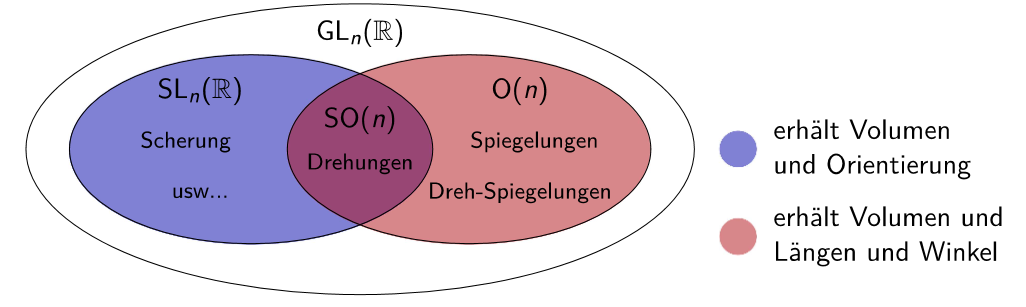
\includegraphics[width=10cm]{papers/clifford/Bilder/MatrizenGruppen.png}
	\caption{Matrizengruppen}
	\label{BildMatrizenGruppen}
\end{figure}

\subsection{Drehung in der geometrische Algebra}
Da wir jetzt aus der Geometrie wissen, dass eine Drehung durch zwei Spiegelungen gebildet werden kann, können wir die Drehung mit der Formel \eqref{RefGA} einfach herleiten.
\begin{satz}
	Durch zwei nacheinander auf einen Vektor $\mathbf{v}$ angewendete Spiegelungen lässt sich eine Drehung 
durch
	\begin{align} \label{rotGA}
\mathbf{v}\mapsto
	\mathbf{v}'' = -\mathbf{wv}'\mathbf{w}^{-1} = -\mathbf{w}(-\mathbf{uvu}^{-1})\mathbf{w}^{-1} = (\mathbf{wu})\mathbf{v}(\mathbf{u}^{-1}\mathbf{w}^{-1})
	\end{align}
	beschreiben.
\end{satz}
Die Vektoren $\mathbf{w}$ und $\mathbf{u}$ bilden hier wiederum die Spiegelachsen. Diese Formel versuchen wir jetzt noch durch Umstrukturierung zu verbessern. 
\subsubsection{Exponentialform}
Dazu leiten wir zuerst die Exponentialform eines Vektors her. Es wird dabei zur Vereinfachung davon ausgegangen, dass alle Vektoren $\mathbf{w}, \mathbf{u}, \mathbf{v}$ in der $\mathbf{e}_{1}$-$\mathbf{e}_{2}$-Ebene liegen. Weitere Drehungen können in höheren Dimensionen durch Linearkombinationen von Drehungen in den $\mathbf{e}_{i}$-$\mathbf{e}_{j}$-Ebenen $(i\not=j)$ erreicht werden. Für die Herleitung ersetzen wir als erstes in der Polarform
\begin{align*}
\mathbf{w} = |\mathbf{w}| \left(\cos(\vartheta_w) \mathbf{e}_1 + \sin(\vartheta_w) \mathbf{e}_2\right)
\end{align*}
eines Vektors einen Faktor 1 durch $1=\mathbf{e}_1^2$ und erhalten beim Sinus
\begin{align}\label{e1ausklammern}
\mathbf{w} &= |\mathbf{w}| \left(\cos(\vartheta_w) \mathbf{e}_1 + \sin(\vartheta_w) \mathbf{e}_1\mathbf{e}_1\mathbf{e}_2\right). 
\end{align}
In einem zweiten Schritt klammern wir $\mathbf{e}_1$ aus, dies ergibt
\begin{align}
\mathbf{w} = |\mathbf{w}|\mathbf{e}_1\left(\cos(\vartheta_w)+ \sin(\vartheta_w) \mathbf{e}_{12}\right). \label{ExponentialGA}
\end{align}
Die Ähnlichkeit des Klammerausdrucks in der Formel \eqref{ExponentialGA} zu der eulerschen Formel bei den komplexen Zahlen ist nun schon gut erkennbar. Versuchen wir nun mithilfe der Reihenentwicklungen
\index{eulersche Formel}%
\index{Reihenentwicklung}%
\begin{align*}
\sin(\vartheta_w)\mathbf{e}_{12}&=\sum _{n=0}^{\infty }(-1)^{n}{\frac {\vartheta_w^{2n+1}}{(2n+1)!}}\mathbf{e}_{12} =\vartheta_w\mathbf{e}_{12}-{\frac {\vartheta_w^{3}}{3!}}\mathbf{e}_{12}+{\frac {\vartheta_w^{5}}{5!}}\mathbf{e}_{12}-\cdots \\
\cos(\vartheta_w)&=\sum _{n=0}^{\infty }(-1)^{n}{\frac {\vartheta_w^{2n}}{(2n)!}} =1-{\frac {\vartheta_w^{2}}{2!}}+{\frac {\vartheta_w^{4}}{4!}}-\cdots
\end{align*}
diesen Zusammenhang auch hier herzustellen. Setzt man diese beiden Reihenentwicklungen in \eqref{ExponentialGA} ein, erhält man
\begin{align*}
\cos(\vartheta_w)+ \sin(\vartheta_w) \mathbf{e}_{12} &= 1+\vartheta_w\mathbf{e}_{12}-{\frac {\vartheta_w^{2}}{2!}}-{\frac {\vartheta_w^{3}}{3!}}\mathbf{e}_{12}+{\frac {\vartheta_w^{4}}{4!}}+{\frac {\vartheta_w^{5}}{5!}}\mathbf{e}_{12}-\cdots
\end{align*}
Dies sieht noch nicht wie eine Exponentialreihe aus, da $\mathbf{e}_{12}$ nur in jedem zweiten Term auftritt.
Da aber $\mathbf{e}_{12}^2=-1$ gibt, erhält man für
\begin{align}
e^{\vartheta_w\mathbf{e}_{12}} = 1 \mathbf{e}_{12}^0+\vartheta_w\mathbf{e}_{12}^1+{\frac {\vartheta_w^{2}}{2!}}\mathbf{e}_{12}^2+{\frac {\vartheta_w^{3}}{3!}}\mathbf{e}_{12}^3+{\frac {\vartheta_w^{4}}{4!}}\mathbf{e}_{12}^4+{\frac {\vartheta_w^{5}}{5!}}\mathbf{e}_{12}^5+\dots.
\label{ExponentialGA2}
\end{align}
Man sieht, dass die beiden Reihen übereinstimmen. Es folgt somit
\begin{align}\label{EulerGA}
e^{\vartheta_w \mathbf{e}_{12}} = \cos(\vartheta_w)+ \sin(\vartheta_w) \mathbf{e}_{12},
\end{align} 
was zeigt, dass es eine Euler-Formel mit $\mathbf{e}_{12}$ anstelle der imaginären Einheit $j$ gibt.

Wenn man jetzt den Vektor \eqref{ExponentialGA} durch die eulersche Schreibweise
\begin{align}
\mathbf{w} = |\mathbf{w}|\mathbf{e}_1e^{\vartheta_w\mathbf{e}_{12}}
\end{align}
ersetzt, kann die Exponentialform des Vektors ähnlich wie die der komplexen Zahlen interpretieren. Der Einheitsvektor $\mathbf{e}_1$ wird um die Länge $|\mathbf{w}|$ gestreckt und um $\vartheta_w$ gedreht.
\subsubsection{Vektormultiplikation}
Nun werden wir das Vektorprodukt
\begin{align} \label{VektorproduktformelGA}
\mathbf{wu} = |\mathbf{w}|\mathbf{e}_1 e^{\vartheta_w \mathbf{e}_{12}}|\mathbf{u}|\mathbf{e}_1 e^{\vartheta_u \mathbf{e}_{12}}
\end{align}
so umformen, dass wir die Drehung nur durch Exponentialterme beschreiben können. Wir tauschen dafür zuerst beim Vektor $\mathbf{w}$ die Reihenfolge von 
$\mathbf{e}_1$ mit dem Exponentialterm $e^{\vartheta_w \mathbf{e}_{12}}$, indem wir bei der Gleichung \eqref{e1ausklammern} $1=\mathbf{e}_1^2$ an einer anderen Position einsetzen.
Wir erhalten
\begin{align*} 
\mathbf{w} &= |\mathbf{w}|\left(\cos(\vartheta_w)+ \sin(\vartheta_w) \mathbf{e}_2\mathbf{e}_1\right)\mathbf{e}_1.
\end{align*}
Mithilfe der Formel \eqref{EulerGA} und dem Wissen, dass $\mathbf{e}_{21}= -\mathbf{e}_{12}$ können wir die Umformung
\begin{align*}
|\mathbf{w}|e^{-\vartheta_w \mathbf{e}_{12}}\mathbf{e}_1
\end{align*}
ausführen. Diese wichtige Umstrukturierung können wir wieder in die Vektorproduktformel \eqref{VektorproduktformelGA} einsetzen und erhalten
\begin{align*}
\mathbf{wu} &= |\mathbf{w}|\,|\mathbf{u}|e^{-\vartheta_w \mathbf{e}_{12}}\mathbf{e}_1\mathbf{e}_1 e^{\vartheta_u \mathbf{e}_{12}}\\
&= |\mathbf{w}|\,|\mathbf{u}|e^{(\vartheta_u-\vartheta_w) \mathbf{e}_{12}}.
\end{align*}
Das inverse Vektorprodukt
\begin{align*}
\mathbf{u}^{-1}\mathbf{w}^{-1} = \dfrac{1}{|\mathbf{w}|\,|\mathbf{u}|}e^{(\vartheta_w-\vartheta_u) \mathbf{e}_{12}}
\end{align*}
kann durch die selbe Methode vereinfacht werden.
Wenn wir den Winkel zwischen den Vektoren  $\mathbf{w}$ und $\mathbf{u}$ als $\vartheta = \vartheta_w - \vartheta_u$ definieren erhalten wir als endgültige Form der Vektorprodukte
\begin{align}\label{wuExpo}
\mathbf{wu} &= |\mathbf{w}|\,|\mathbf{u}|e^{-\vartheta \mathbf{e}_{12}}\enspace\text{und}\\
\mathbf{u}^{-1}\mathbf{w}^{-1} &= \dfrac{1}{|\mathbf{w}|\,|\mathbf{u}|}e^{\vartheta \mathbf{e}_{12}} \label{wuExpoInv}.
\end{align}
\subsubsection{Umstrukturierte Drehungsgleichung}
Setzten wir nun unsere neuen Erkenntnisse in die Gleichung \eqref{rotGA} ein, erhalten wir
\begin{align*}
\mathbf{v''}
=
(|\mathbf{w}|\,|\mathbf{u}|e^{-\vartheta \mathbf{e}_{12}})\mathbf{v}\biggl(\dfrac{1}{|\mathbf{w}|\,|\mathbf{u}|}e^{\vartheta \mathbf{e}_{12}}\biggr)
\end{align*}
und können durch die Kürzungen der Längen die vereinfachte Drehungsgleichung
\begin{align} \label{GAvereinfRot}
\mathbf{v''} = e^{-\vartheta \mathbf{e}_{12}} v e^{\vartheta \mathbf{e}_{12}}
\end{align}
bilden.
Wir wissen nun, dass diese beidseitige Multiplikation die Länge von $\mathbf{v}$ nicht verändert, da sich die Längen von $\mathbf{w}$ und $\mathbf{u}$ kürzen.

Betrachten wir nun den Effekt der Exponentialterme auf $\mathbf{v}$. Dabei teilen wir den Vektor $\mathbf{v}$ auf in einen Anteil $\mathbf{v_\parallel}$, welcher auf der Ebene $\mathbf{e}_{12}$ liegt, und einen Anteil $\mathbf{v_\perp}$, welcher senkrecht zu der Ebene steht. Wir bekommen durch Einsetzten nun die Form
\begin{align} \label{RotAufPerpPar}
\mathbf{v}'' = e^{-\vartheta \mathbf{e}_{12}} (\mathbf{v_\perp + v_\parallel}) e^{\vartheta \mathbf{e}_{12}} = e^{-\vartheta \mathbf{e}_{12}} \mathbf{v_\perp} e^{\vartheta \mathbf{e}_{12}} + e^{-\vartheta \mathbf{e}_{12}} \mathbf{v_\parallel} e^{\vartheta \mathbf{e}_{12}}.
\end{align}
Auf eine allgemeine Herleitung wird hier zwar verzichtet, aber man kann zeigen, dass man die Reihenfolge der Vektoranteile $\mathbf{v_\perp}$ und $\mathbf{v_\parallel}$ mit dem Exponentialterm $e^{-\vartheta \mathbf{e}_{12}}$ so vertauschen kann, dass sich 
\begin{align*}
\mathbf{v}'' = \mathbf{v_\perp} e^{-\vartheta \mathbf{e}_{12}}  e^{\vartheta \mathbf{e}_{12}} +  \mathbf{v_\parallel} e^{-(-\vartheta) \mathbf{e}_{12}} e^{\vartheta \mathbf{e}_{12}}
\end{align*}
ergibt. Der Winkel wird beim parallelen Anteil negiert. An der zusammengefassten Gleichung
\begin{align}\label{RotParPerp}
\mathbf{v}'' = \mathbf{v_\perp} +  \mathbf{v_\parallel} e^{2\vartheta \mathbf{e}_{12}}
\end{align}
kann man sehen, dass nur der parallele Anteil $\mathbf{v_\parallel}$ des Vektors $\mathbf{v}$ in der Ebene $\mathbf{e}_{12}$ um $2\vartheta$ gedreht wird.
Der senkrechte Anteil $\mathbf{v_\perp}$ bleibt gleich.
Wichtig dabei zu sehen ist, dass nur der Winkel zwischen den Vektoren $\mathbf{w}$ und $\mathbf{u}$ von Bedeutung ist.
Die Länge und Richtung der einzelnen Vektoren spielt keine Rolle.
Wir zeigen nun diese Eigenschaften an einem Beispiel.

\begin{beispiel} 
	Gegeben sei ein Vektor $\mathbf{v} = 1\mathbf{e}_1 + 2\mathbf{e}_2 + 3\mathbf{e}_3$ mit zur $\mathbf{e}_{12}$-Ebene parallelen Anteil $\mathbf{v_\parallel} = 1\mathbf{e}_1 + 2\mathbf{e}_2$ und senkrechten Anteil $\mathbf{v_\perp} = 3\mathbf{e}_3$. Zusätzlich sind die Spiegelachsen $\mathbf{u} = \mathbf{e}_1$ und $\mathbf{w} = 2\mathbf{e}_2$ gegeben. Gesucht ist der gedrehte Vektor $\mathbf{v}''$. Bestimmen wir als erstes das Vektorprodukt
	\begin{align*}
	\mathbf{wu} = (2\mathbf{e}_2)(\mathbf{e}_1) = -2\mathbf{e}_{12}
	\end{align*}
	und das Produkt der Inversen
	\begin{align*}
	\mathbf{u}^{-1}\mathbf{w}^{-1} = \biggl(\dfrac{\mathbf{e}_1}{1^2}\biggr) \biggl(\dfrac{2\mathbf{e}_2}{2^2}\biggl) = \dfrac{1}{2}\mathbf{e}_{12}.
	\end{align*}
	Den gedrehten Vektor $\mathbf{v}''$ können wir nun durch Einsetzen und Auflösen der Produkte in die Gleichung \eqref{rotGA} bestimmen. Der Rechnenvorgang ist
	\begin{align*}
	\mathbf{v}'' = (\mathbf{wu})\mathbf{v}(\mathbf{u}^{-1}\mathbf{w}^{-1}) &= (-2\mathbf{e}_{12})(1\mathbf{e}_1 + \mathbf{e}_2 + 1\mathbf{e}_3)(\textstyle{\frac{1}{2}}\mathbf{e}_{12})\\
	&= (2\mathbf{e}_2-2\mathbf{e}_1-2\mathbf{e}_{123})(\textstyle{\frac{1}{2}}\mathbf{e}_{12})\\
	&= -1\mathbf{e}_1 - 1\mathbf{e}_2 + 1\mathbf{e}_3.
	\end{align*}
	Aus dem Resultat $\mathbf{v}''= -1\mathbf{e}_1 + 1\mathbf{e}_2 + 1\mathbf{e}_3$ können wir bestätigen, dass
	\begin{itemize}
		\item die Länge $|\mathbf{v}| = \sqrt{3}$ zur Länge $|\mathbf{v}''|=\sqrt{3}$ gleich blieb.
		\item sich der parallele Anteil $\mathbf{v_\parallel}'' = -1\mathbf{e}_1 - 1\mathbf{e}_2$ gedreht hat und der senkrechte Anteil $\mathbf{v_\perp}'' = 1\mathbf{e}_3$ unverändert blieb.
		\item der parallele Teil sich genau um $2\vartheta=180^\circ$ gedreht hat. $\vartheta$ kann übrigens durch die Umformung des Produkt $\mathbf{wu}$ in die Exponentialschreibweise
		\begin{align}
		&\mathbf{wu} = -2\mathbf{e}_{12} = 2(0-1\mathbf{e}_{12})=2(\cos\biggl(\dfrac{-\pi}{2}\biggr) + \sin\biggl(\dfrac{-\pi}{2}\biggr)\mathbf{e}_{12}) = 2e^{(-\pi/2)\mathbf{e}_{12}}
		\end{align}
		durch einen Vergleich mir der Formel \eqref{wuExpo} als
		\begin{align*}
		\vartheta = -\biggl(\dfrac{-\pi}{2}\biggr) = \dfrac{\pi}{2}
		\end{align*}
		ausgelesen werden. \qedhere
	\end{itemize}
\end{beispiel} 
